\chapter{Introduction}

\epigraph{``And now you're asking, I don't know where to begin''}{{\sl Mike Vennart, Silent/Transparent}}
%
%“We demand rigidly defined areas of doubt and uncertainty!” 
%― Douglas Adams, The Hitchhiker's Guide to the Galaxy

The release of gravitational potential energy as mass falls towards
a compact object is the most efficient energetic process in the universe,
capable of liberating more rest mass energy than nuclear fusion.
This {\em accretion} process is thought to power the huge radiative engines at the 
centres of every galaxy -- accreting supermassive black holes known as active galactic nuclei (AGN).
As the matter falls into the potential well of the black hole it often forms an accretion disc,
which, in many cases, is an efficient radiator of the gravitational energy released.
In some cases, the accretion disc can outshine the entire stellar population of the galaxy,
appearing as a quasi-stellar object (QSOS) or {\em quasar} 
In addition to AGN, accretion discs are present in X-ray binaries (XRBs), young-stellar objects (YSOs) and
cataclysmic variables (CVs). Accretion therefore appears to be a universal process; 
broadly speaking, the physics is similar regardless of 
whether matter is falling on to a $\sim1~M_\odot$ Neutron Star or White Dwarf 
system, or a $\sim10^{10}~M_\odot$ black hole. 

Outflows are ubiquitous in accreting systems. We see collimated radio jets in AGN (REF) and
XRBs (REF), and there is even evidence of extended radio emission in AWDs (REF). These radio jets
tend to appear in specific accretion states (REF), implying an intrinsic connection to the 
accretion process. Even more intriguing, in XRBs less collimated, mass-loaded outflows
or {\em winds} are observed in the opposite accretion state, possibly emanating from the accretion disc.
Evidence for disc winds is widespread across the mass range, but perhaps the most spectacular indication
is the blue-shifted, broad absorption lines (BALs) in the rest-frame ultraviolet (UV)
seen in high-state CVs (REFs) 
and the so-called broad absorption line quasars that make up $20-40\%$
of quasars (BALQSOs; REFs). These BALs are also seen in O-stars (REFs) and sometimes even
in the optical spectra of CVs (REFs). 
Broad, blue-shifted absorption is also observed in the Fe K$\alpha$ line in 
AGN (REFs) -- these are often known
as ultra-fast outflows or UFOs\footnote{It should be noted that, while X-ray spectral
fitting can be somewhat of a dark art, the explanations for these
UFOs are somewhat more believable than their sci-fi namesakes.}.

The astrophysical significance of disc winds extends, quite literally, 
far beyond the accretion environment. They offer a potential mechanism by which the central
accretion engine can interact with the host galaxy and interstellar medium (REFs). 
This is often referred to as AGN feedback (REF), and is required in models of 
galaxy evolution. Furthermore, winds offer a natural way to {\em unify} much
of the diverse phenomenology of AGN, CVs and XRBs. The principle of unification
can be applied along more than one `axis' of parameter space. For example, 
there exist elegant models that attempt to explain {\em all}
of the behaviour of quasars with only a central black hole, a jet, an accretion disc,
and an associated outflow, by varying the viewing angle.
Similarly elegantly, it has been shown that much of the behaviour of XRBs
is directly applicable to AGN (REFs), and models of outflows in CVs have been successfully

Despite their clear importance and ubiquity, there are still
many unanswered questions relating to the true impact of winds and their underlying
physical origins. Here, I aim to address some of these questions, and 
take steps towards building a more holistic picture of the impact
of winds on the spectral appearance and accretion physics of disc systems.
This thesis is structured as follows. In the remainder of this chapter, 
I will give the background accretion theory 
and detail the successes and failures of accretion disc models when compared to observations,
as well as describing the different classes of accreting objects in more detail. 
In chapter 2, I dedicate some time to specifically discussing the theory of,
and observational evidence for, accretion disc winds. In chapter 3, I outline 
the Monte Carlo radiative transfer (MCRT) and photoionization
methods I have used in order to investigate the impact of disc 
winds on the spectra of accreting systems. The science chapters
contain three separate submitted papers, in which we investigated the impact
of disc winds on the spectra of CVs (Chapter 5), and tested disc wind
quasar unification models (Chapters 6 and 7).
In chapter 8, I summarise my findings and their astrophysical significance, 
and discuss potential avenues for future work.


\section{The Physics of Accretion}

The basic phenomenon of accretion- matter falling into a gravitational potential well- 
is a ubiquitous one in astrophysics. 


\subsection{Roche Lobe-Overflow}

In binary systems, there are only two ways by which matter can transfer 
from the secondary to the compact object. One is by Roche Lobe-overflow (RLOF),
whereby stellar evolution causes the donor star to fill it's Roche Lobe, the surface
of equipotential around the star. The alternative is that a radiatively driven wind
may expel stellar material from the donor, allowing some of it to flow onto the compact object.
Although stellar wind accretion is common in some classes (REFs), here I will focus on 
RLOF as it is more common in the systems that commonly exhibit high-state accretion discs
and associated outflows.

The Roche potential, $\Phi_R$, can be expressed as ?



\subsection{Accretion discs}

The basic phenomenon of accretion- matter falling into a gravitational potential well- 
is a ubiquitous one in astrophysics. The details of how and where the energy is released
and how angular momentum is transported is subject to a number of different 
interpretations, mainly depending on the {\em geometry} of the accretion flow.




The so-called $\alpha$-disc model developed by \cite[][hereafter SS73]{shakurasunyaev1973} is
currently the leading candidate for explaining how energy and angular momentum
is transported an accretion disc. The starting point for this model is the parameterisation
of viscosity using a simple form of
\begin{equation}
\nu = \alpha c_s H.
\end{equation}
Viscous torques then allow the conversion of orbital kinetic energy into heat, which 


By considering the energy released through viscous dissipation 
in the disc it is possible to derive a temperature distribution as a function of 
radius \citep{shakurasunyaev1973, fkrbook}. 

\begin{equation}
T(R) =  
\end{equation}

It is important to recognise that the work of \cite{shakurasunyaev1973} 
{\sl does not specify the nature of the disc SED}. What it does do is 
say where energy is originally released. Typically,
accretion discs are modelled as a series of annuli each emitting 
as blackbodies, but it is possible that a disc atmosphere with frequency-dependent
opacity would create a somewhat different spectrum. It is also possible that {\em neither} of these 
treatments are realistic. We shall therefore devote a little time to discussing
the observational arguments for accretion discs and the current problems 


\section{Observational Appearance}


\section{Accreting Compact Binaries}

\subsection{Cataclysmic Variables}

Cataclysmic variables (CVs) are systems in which a white dwarf
accretes matter from a donor star via Roche-lobe overflow. 
In non-magnetic systems this accretion is mediated by a Keplerian disc
around the white dwarf (WD). Nova-like variables (NLs) are a subclass
of CVs in which the  disc is always in a relatively
high-accretion-rate state ($\dot{M} \sim 10^{-8}$~M$_{\odot}$~yr$^{-1}$).  
This makes NLs an excellent laboratory for studying the properties of 
steady-state accretion discs. 

\subsection{X-ray Binaries}
X-ray binaries are similar to CVs in structure, except that the compact object
is either a neutron star (NS) or black hole (BH). The accretion disc 
emits in the soft X-rays, and an additional hard X-ray power law is also 
seen in the spectrum (REFs). This hard component is normally attributed
to Compton up-scattering of seed disc photons by some kind of `corona'
of hot electrons close to the BH (REFs). 

Although I do not discuss XRBs directly in this thesis, it is instructive
to discuss some of their observational appearance as it is instructive 
for understanding the theory of disc winds, as well as their wider significance. 
The discovery that XRBs follow similar tracks on a hardness-intensity diagram (REFs)
is particularly interesting in this regard, especially since Ponti et al. (2012)
showed that broad Fe absorption lines are only seen in the soft-state 
high-inclination systems, implying that equatorial outflows are intrinsic to 
the accretion process (see figure~\ref{fig:ponti_cartoon}). Although the driving mechanism
is almost certainly different to CVs (REFs), the similarity in general structure 
to models for CVs and quasars is striking.

\begin{figure}
\centering
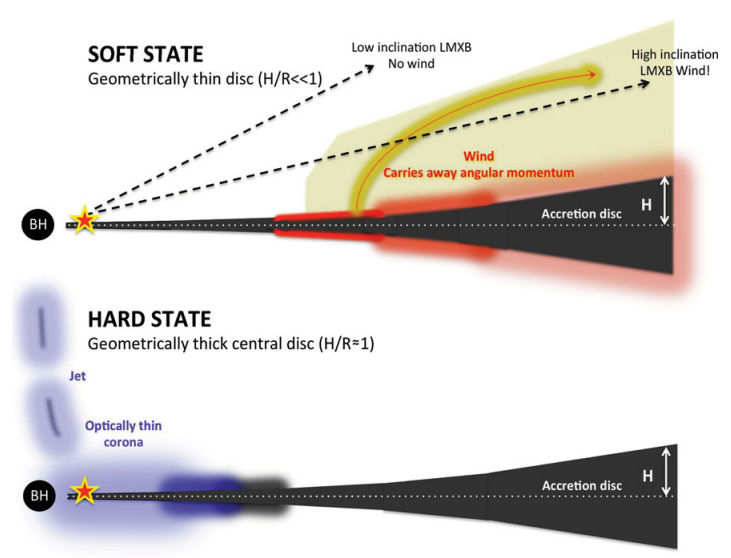
\includegraphics[width=0.7\textwidth]{figures/01-intro/ponti_wind_cartoon.png}
\caption
[Hardness intensity diagram for a WD, NS and BH system]
{
{\sl Credit: Ponti et al. 2012}
Hardness intensity diagram for a WD, NS and BH system
} 
\label{fig:ponti_cartoon}
\end{figure}


\section{Quasars and Active Galactic Nuclei}

Spectra of AGN have now been studied for over 100 years, and we have known 
that they exhibit strong, broad emission lines since the first spectrum was taken by
\cite{fath1909}.
However, it wasn't until the work of \cite{seyfert1943} that the systematic 
classification of AGN really began, leading to the phrase `Seyfert galaxy'.
This label was applied to galaxies possessing a bright nucleus, spectroscopically
characterised by a blue continuum and a series of strong emission lines.
The first real physical insight into the extraordinary nature of AGN
was provided by \cite{woltjer1959}, who noted that (i) the nuclei must have sizes $<100$~pc,
based on the fact that they were unresolved and (ii) the mass of the nucleus
must be very high, based on virialised motion. 
While both of these observations were based on simple arguments, the fact that these
ultra-luminous celestial objects are both {\em compact} and {\em supermassive}
is perhaps the defining insight into the nature of AGN.

Although the field of AGN study was established in the optical, 
radio astronomy also significantly furthered our understanding of AGN
in the mid-20th century. A number of surveys, such as the Cambridge \citep{edge1959}, 
Parkes \citep{ekers1969} and Ohio \citep{ehman1970} surveys discovered a great many 
bright radio point sources distributed isotropically across the sky.
These sources eventually became known as `quasi-stellar radio sources'
or {\em quasars}, and were soon identified to be coincident with bright optical
sources or `quasi-stellar objects' (QSOs; REFs). 
Nowadays, the term quasar normally has very little to do with 
radio emission and is often used interchangeably with QSO. 
Indeed, throughout this thesis I shall refer to a quasar as simply a bright, 
massive AGN; one with sufficiently high luminosity that it dominates the emission 
from it's host galaxy. 

\subsection{AGN Unification and the dusty Torus}

Although Seyfert had identified type 1 and 2 AGN, a physical explanation
for this dichotomy was not forthcoming until a seminal study by \cite{antonucci1985}.
They showed unambiguously that the nearby Seyfert 2 NGC~1068 is simply an obscured
type 1 AGN, by finding that broad emission lines appeared in the spectrum of
{\em polarised} flux. This provided the basis for the first successful attempt
to unify AGN behaviour (REF), as it elegantly explained the apparent disconnect between
the two types of AGN as simply a viewing angle effect. The obscuring structure became known as 
the `torus' \citep{krolik1986}, due to its geometry, and it was soon realised that this structure
may be made of dust (REF), in which case it could also be responsible for the infra-red (IR)
bump in AGN \citep{neugebauer1979}. 
Since then, the picture has become somewhat more complicated. Dusty polar outflows
have been found to be important IR emitters (REFs) and changing-look 
AGN have been discovered (REFs), as just a couple of examples.
Nevertheless, the AGN unification picture still helps explain a lot of AGN spectral components,
and represents a good framework to test with observations. 

\subsection{The Broad Line Region and Connection to Outflows}

Within the 

As noted by \cite[][hereafter MCGC95]{MCGV95}, there are a number of problems with
the BLR `cloud' model, perhaps most notably that there is no obvious 
physical origin for a series of virialised clouds. While there are exceptions
to this statement (REFs), it is important to test other models.
Indeed, MCGV95 proposed a disc wind model in order to explain both BALs and BELs
in quasars. A disc wind model was also  discussed by \cite{elvis2000}, 
who proposed a structure for quasars that attempted to explain much 
of the behaviour of luminous AGN
merely as a function of viewing angle. Outflow models are discussed further in section~?.
The philosophy of these models is that, before invoking additional
degrees of freedom in a model, we should first test if known quasar phenomenology 
(winds) can explain other aspects of their observational appearance.
I have illustrated this general principle with the `Occam's quasar' 
cartoon shown in figure~\ref{fig:occam}. This is the picture that I will
to test in the latter, quasar-focused sections of this thesis, and the general
principle can even be applied to cataclysmic variables and other accreting objects.


\begin{figure}
\centering
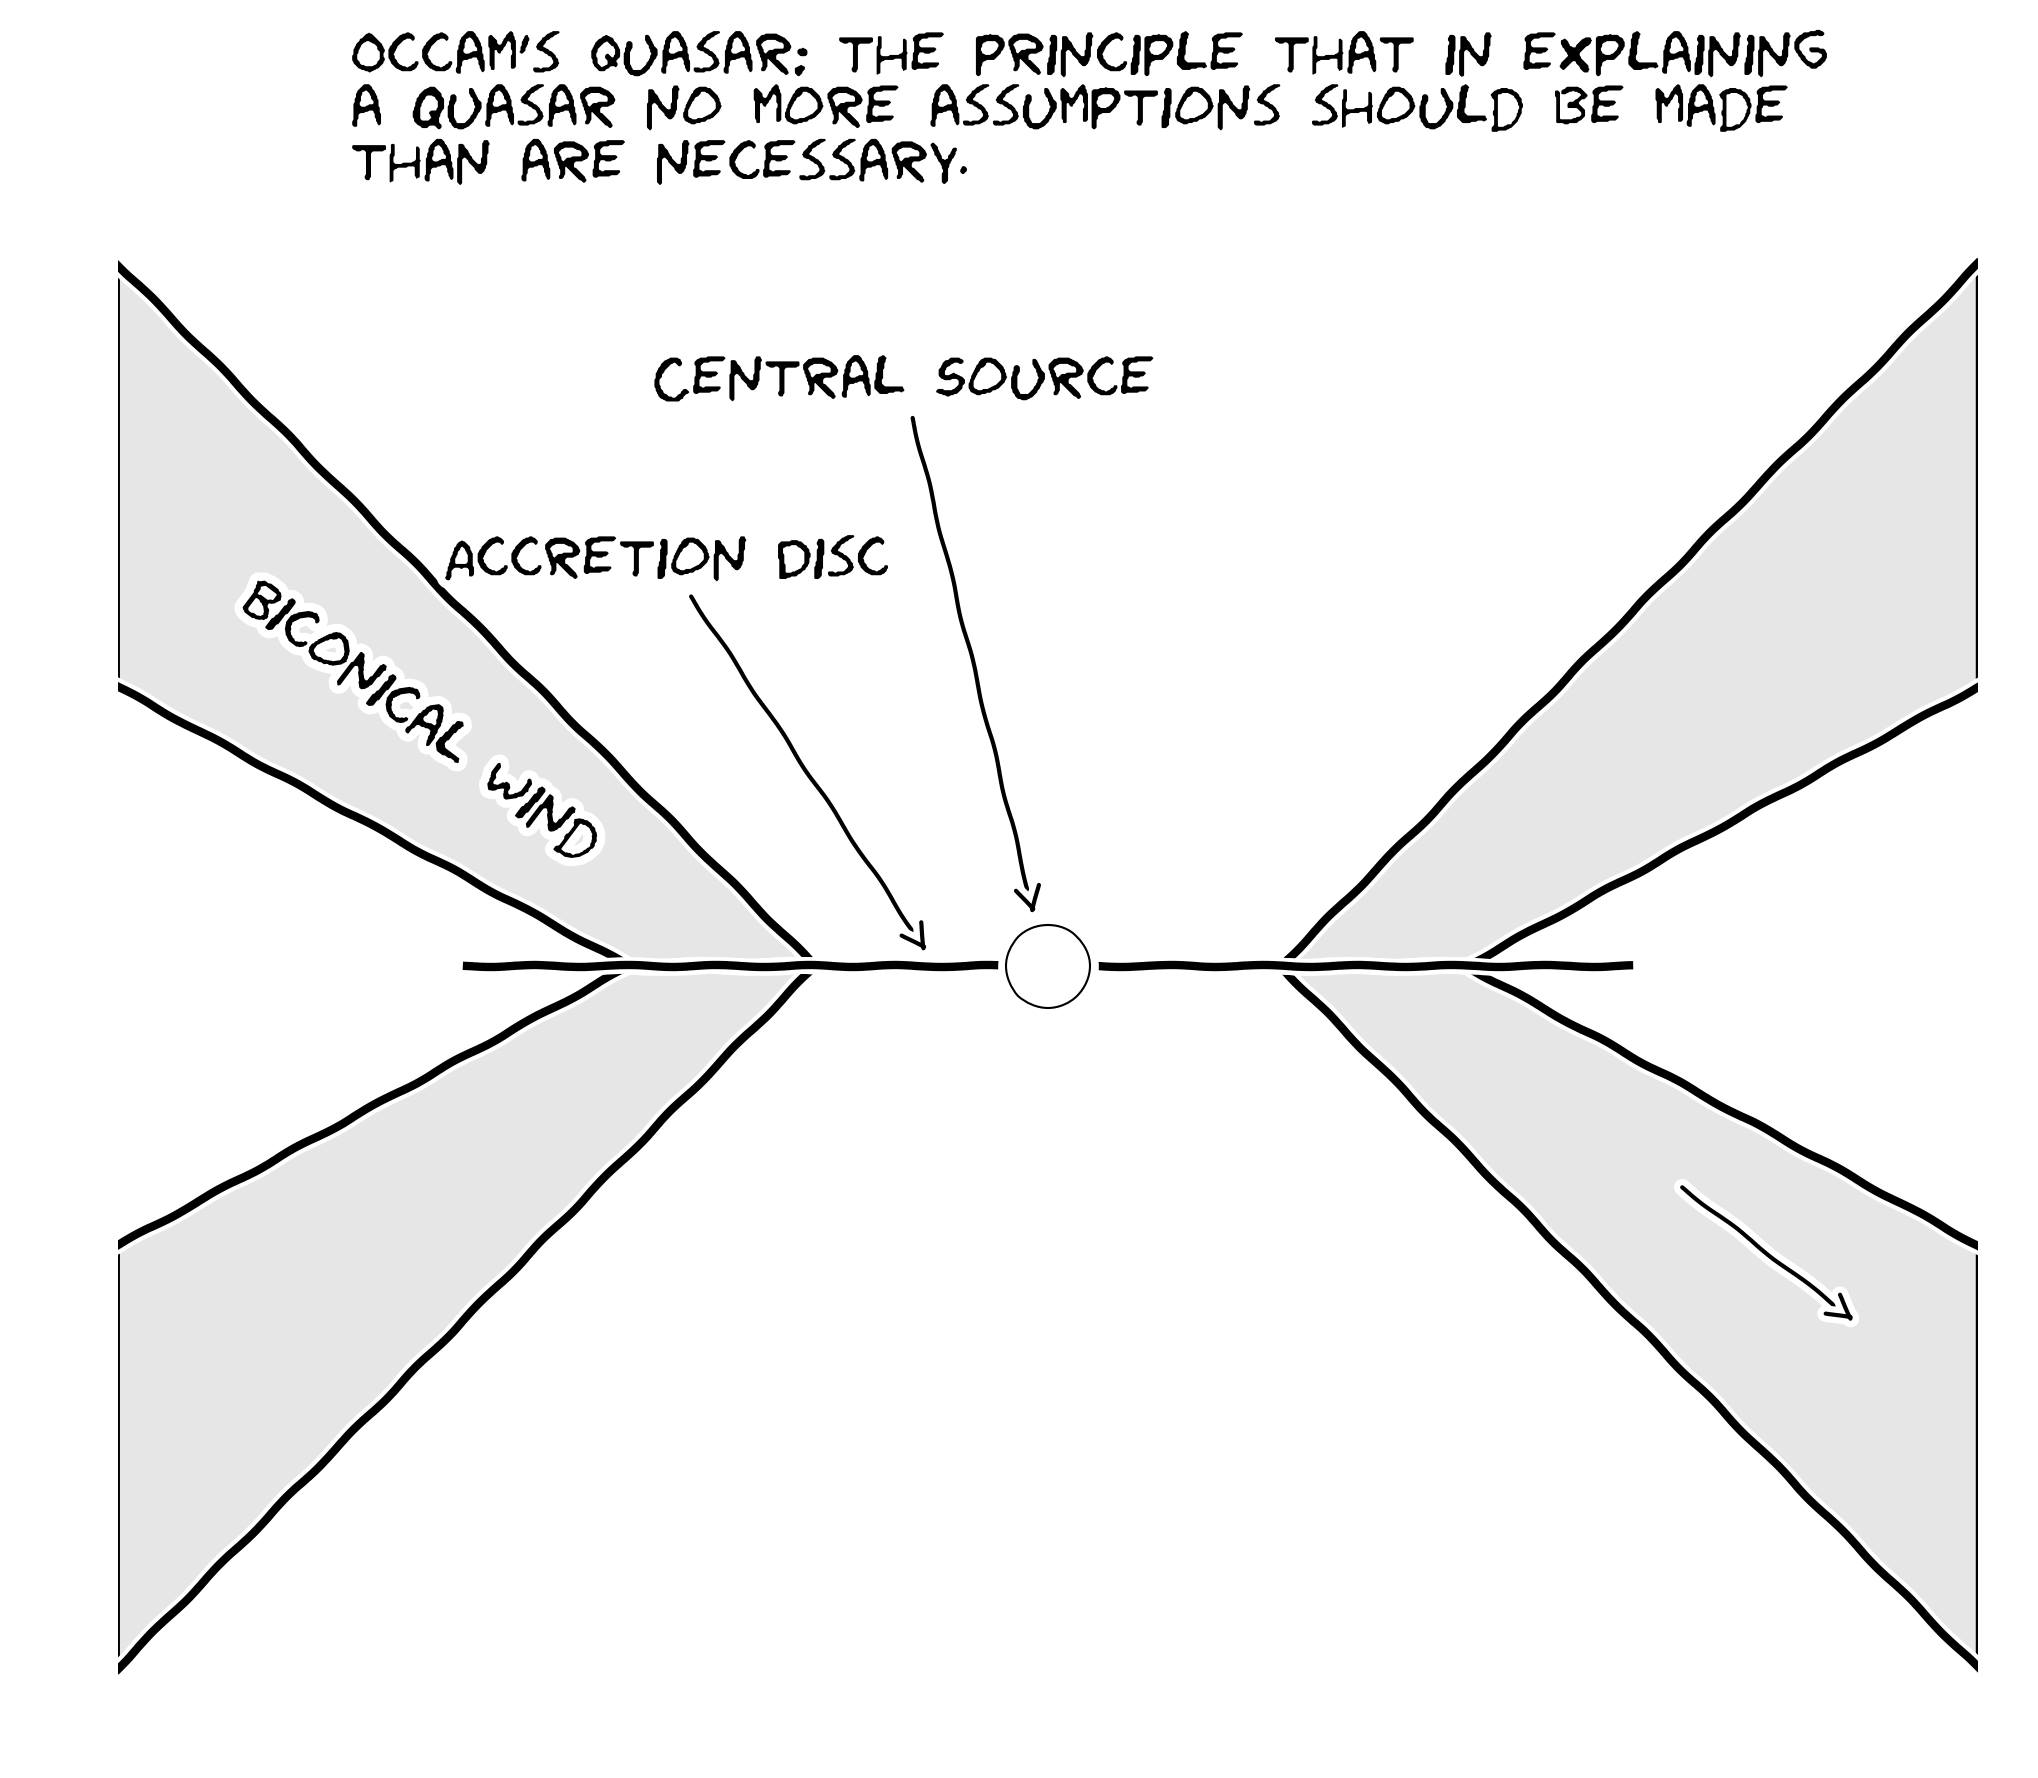
\includegraphics[width=1.0\textwidth]{figures/01-intro/occam.jpg}
\caption
[Occam's quasar]
{
Occam's quasar. How far can this general picture take us when trying to explain
the behaviour of quasars and other accreting compact objects?
} 
\label{fig:occam}
\end{figure}


\subsubsection{Potential Problems with the Thin-disc model}

A number of issues have been raised with the thin-disc model and
its applicability to accreting systems. 

\subsubsection{The Accretion Disc Size Problem}

\subsubsection{The Spectral shape of CV discs}

Attempts to fit the observed SEDs of high-state CVs with simple disc models have met with mixed success. In
particular, the SEDs predicted by most stellar/disc atmosphere models 
are too blue in the UV \citep{wade1988,long1991,long1994,knigge1998} and exhibit
stronger-than-observed Balmer jumps in absorption 
\citep{wade1984,haug1987,ladous1989b,knigge1998}. One possible
explanation for these problems is that these models fail to capture
all of the relevant physics. Indeed, it has been argued that a
self-consistent treatment can produce better agreement with 
observational data (e.g. Shaviv et al. 1991;  but see also Idan et al. 2010).
\nocite{idanshaviv2010} \nocite{shaviv1991}
However, an alternative explanation, suggested by Knigge et al.
(1998b; see also Hassall et al. 1985)\nocite{KLWB98,hassall}, 
is that recombination continuum emission from the base of the 
disc wind might fill in the disc's Balmer absorption edge and flatten the UV spectrum.








\section{The Universality of Accretion}

Accretion appears to be an important physical processes across $\sim9$ orders
of magnitude in mass. But is this process the same at all scales? Does any 
behaviour manifest in all accretion systems? 

\subsection{The RMS-flux relation}

Broad-band variability is common in all types of accretion disc. It has been
known for sometime that there exists a linear relationship
between the flux and absolute root-mean-square (rms) amplitude
of this variability. This was discovered first in XRBs and AGN 
\citep{uttley2001, uttley2005, heil2012}, but it has been shown
more recently that the relationship extends to AWDs and even YSOs 
\citep{scaringi2012,scaringi2015a}. The relationship is not limited
to one type of AWD, as it is present in both NLs and DNe \citep{vandesande2015}.
 
The model that best reproduces this behaviour is the so-called
`fluctuating accretion disc' model (REFs). It has been shown that 
additive processes cannot reproduce the behaviour, and a multiplicative
mechanism is required (REFs). 
Regardless of the mechanism, the rms-flux relation is one of the most
clear-cut examples of a universal accretion phenomenon. 
It tells us that at least some of the behaviour in AWD discs
is present in AGN and XRB, strengthening the argument that AWDs
should be used as `accretion laboratories'. 


\subsection{Accretion States}


\begin{figure}
\centering
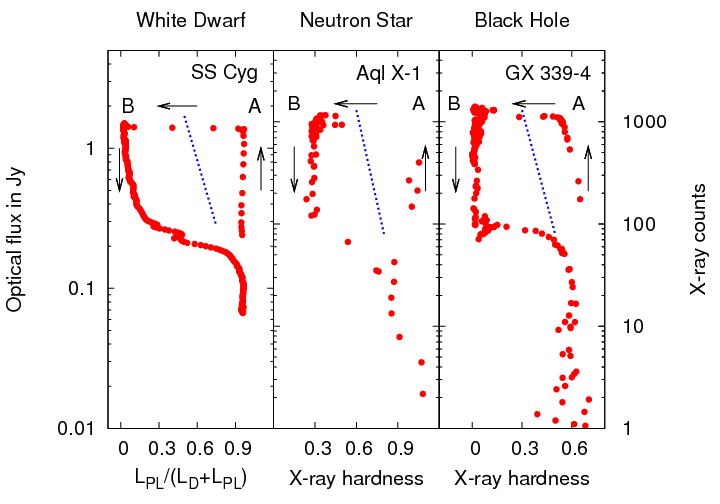
\includegraphics[width=0.7\textwidth]{figures/02-accretion/kording_hid.png}
\caption
{
{\sl Credit: Kording et al. XXXX.} 
Caption.
} 
\label{fig:kording_hid}
\end{figure}



\subsection{Jets and Outflows}


\subsection{A Global Picture}

Clearly, accretion physics is relevant to a plethora of astrophysical phenomena. 
It would also appear that the outflowing material observed in accreting systems 
has a profound effect on the accretion process itself, as well as acting 
as a spectral `filter' -- modifying, and sometimes dominating the observational 
appearance of accretion discs.

